\documentclass{standalone}
\usepackage{tikz,color}
\begin{document}
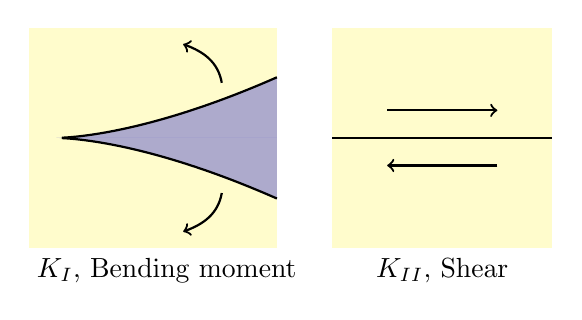
\begin{tikzpicture}[scale=0.7]

\path [fill=blue ,opacity=0.4]
plot [domain=1:40, samples=30, thick ] ( {0.1*\x}, {-0.003*pow(\x,1.6)})
|- (0,0);

\path [fill=blue ,opacity=0.4]
plot [domain=1:40, samples=30, thick ] ( {0.1*\x}, {0.003*pow(\x,1.6)})
|- (0,0);

\path[fill=yellow, opacity=0.2] (-0.5,-2) rectangle (4,2);

\draw [domain=1:40, samples=30, thick] plot( {0.1*\x}, {0.003*pow(\x,1.6)});
\draw [domain=1:40, samples=30, thick] plot( {0.1*\x}, {-0.003*pow(\x,1.6)});

\draw [thick, ->] (3,1) [out = 100, in = 340] to (2.3,1.7);
\draw [thick, ->] (3,-1) [out = 260, in = 20] to (2.3,-1.7);


\path[fill=yellow, opacity=0.2] (5,-2) rectangle (9,2);
\draw [thick] (5,0) to (9,0);
\draw [thick, ->] (6,0.5) to (8,0.5);
\draw [thick, ->] (8,-0.5)to (6,-0.5);

\node at (2,-2) [below] {$K_I$, Bending moment};
\node at (7,-2) [below] {$K_{II}$, Shear};

\end{tikzpicture}
\end{document}
